\documentclass[12pt,a4paper]{article}
\usepackage[T1]{fontenc}
\usepackage[utf8]{inputenc}
\usepackage{lmodern}
\usepackage[left=2.5cm,right=2.5cm,top=2.3cm,bottom=2.3cm]{geometry}
\usepackage{graphicx,booktabs,tabularx,array,xcolor}
\usepackage{microtype,fancyhdr,enumitem,listings,caption,xurl,pdfpages,eso-pic}
\usepackage[unicode,hidelinks]{hyperref}
\hypersetup{pdftitle={Laporan Praktikum Web Service Sesi 11},pdfauthor={Bambang Herlambang},pdfsubject={Dokumentasi API otomatis dan penerapan Auth + Gateway}}
\pagestyle{fancy}\fancyhf{}\fancyfoot[C]{\thepage}
\renewcommand{\headrulewidth}{0pt}
\setlength{\headheight}{15pt}
\setlength{\parindent}{0pt}\setlength{\parskip}{5pt}
\setlength{\emergencystretch}{3em}
\newcolumntype{Y}{>{\raggedright\arraybackslash}X}
\renewcommand{\arraystretch}{1.15}
\setlist{nosep,leftmargin=1.4em,topsep=3pt}
\newcommand{\code}[1]{{\small\nolinkurl{#1}}}
\lstset{basicstyle=\small\ttfamily,breaklines=true,columns=fullflexible,keepspaces=true,showstringspaces=false,frame=single,aboveskip=6pt,belowskip=6pt}
\renewcommand{\figurename}{Gambar}
\captionsetup{font=small,labelfont=bf,labelsep=period}
\begin{document}
\hypersetup{pageanchor=false}

\includepdf[pages=1-14,pagecommand={\thispagestyle{empty}},fitpaper=true]{base-report-16p.pdf}
\hypersetup{pageanchor=true}
\setcounter{page}{14}
\begin{center}
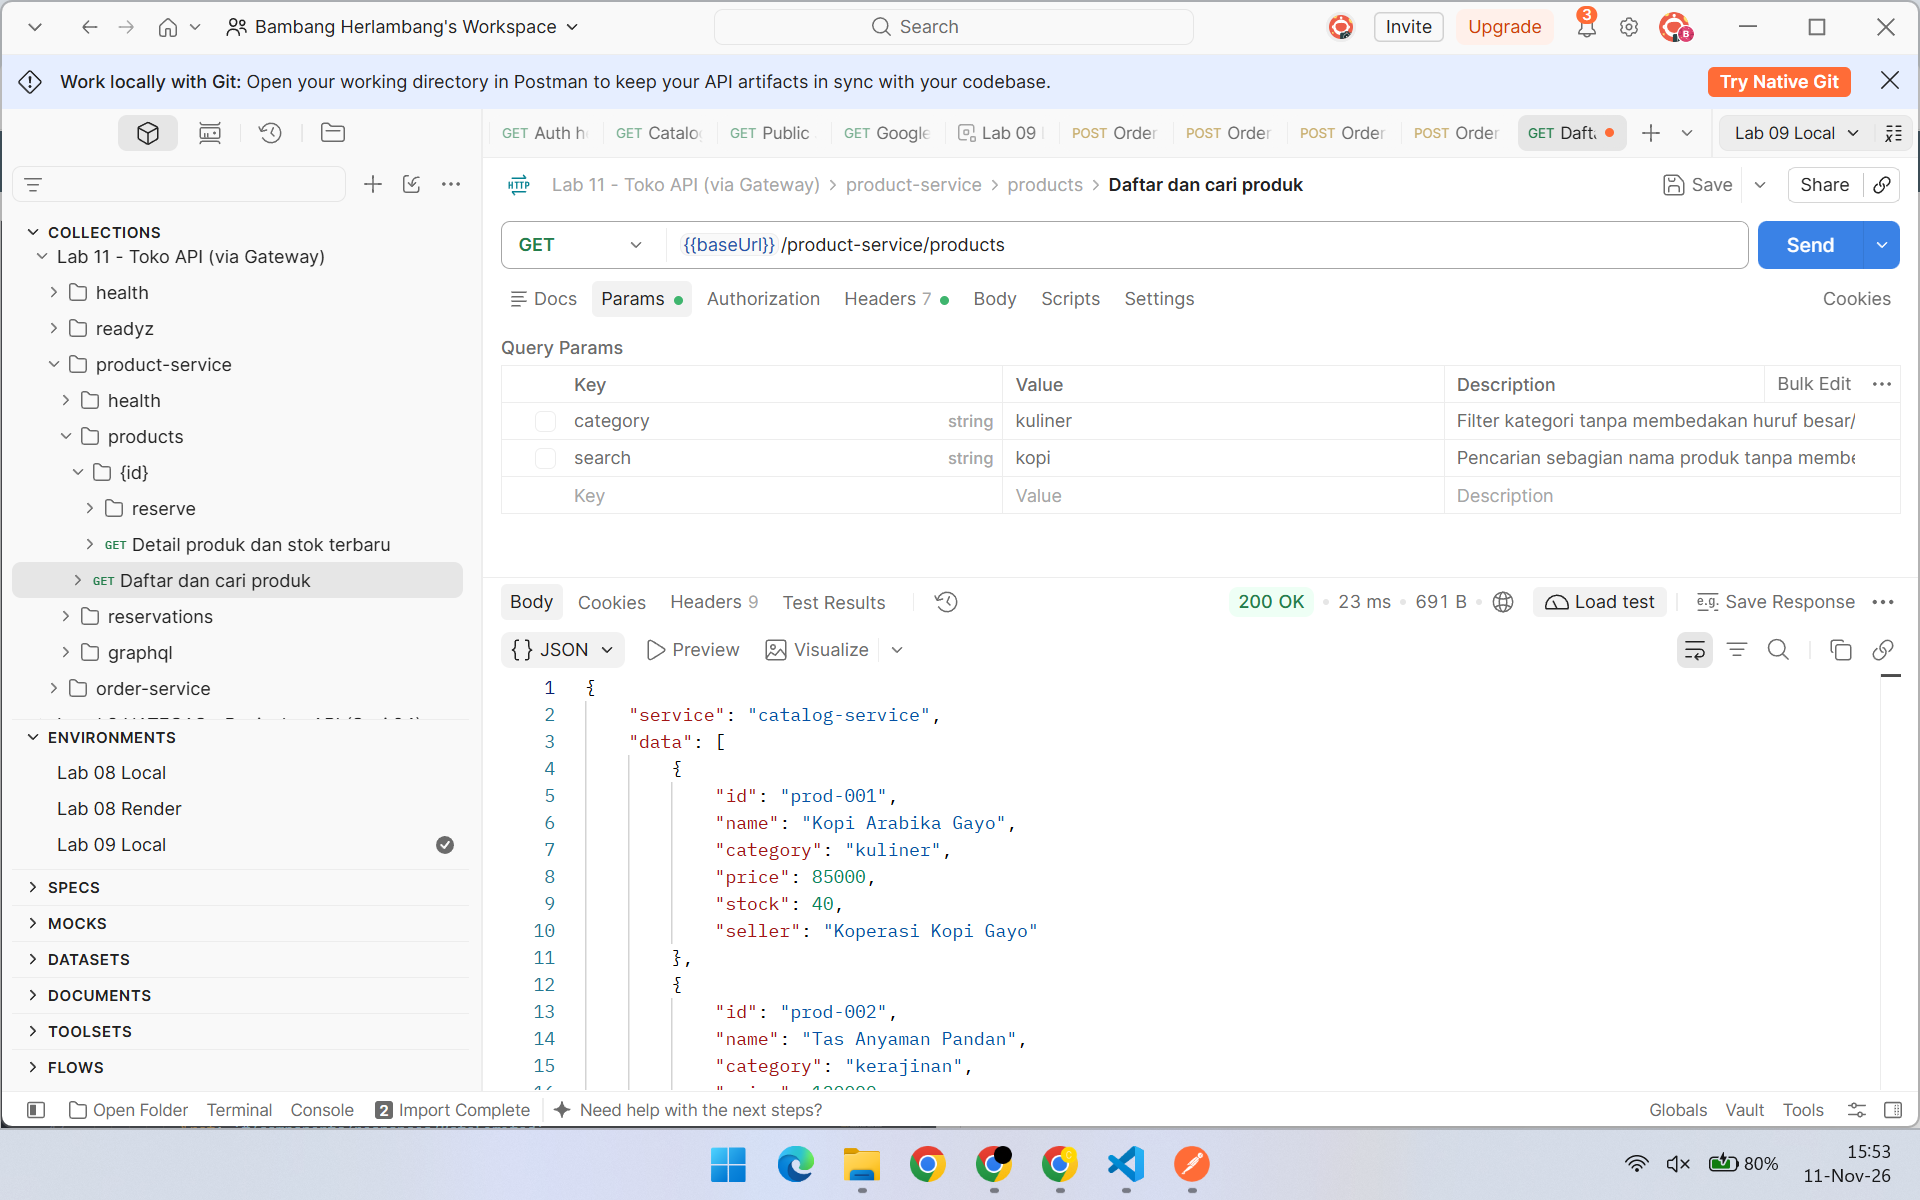
\includegraphics[width=\linewidth,height=8.1cm,keepaspectratio]{images/postman-200.png}
\setcounter{figure}{9}
\captionof{figure}{Hasil aktual request Postman sesudah impor OpenAPI. Sumber: Screenshot (1990).png.}
\end{center}

Koleksi JSON hasil konverter tersedia pada folder \code{docs/postman/} sebagai \code{lab11.postman_collection.json}. Bukti manual berasal dari impor OpenAPI langsung. Status impor yang belum diverifikasi pada rekaman demo otomatis dipertahankan sebagai riwayat saat demo dijalankan; status manual terbaru dan hash screenshot tersimpan dalam \code{verification.json} pada folder \code{docs/evidence/lab11/manual/}.

\setcounter{section}{5}
\section{Penerapan ke proyek: Auth + Gateway}
Komponen individual Bambang Herlambang (5803024019) pada proyek Marketplace UMKM Lokal adalah \textbf{Auth + Gateway}. Untuk penerapan Lab 11, tiga endpoint Auth yang sudah tersedia dalam kode proyek didokumentasikan secara khusus: POST \code{/auth/token}, GET \code{/.well-known/jwks.json}, dan GET \code{/auth/me}.

Spesifikasi mandiri disimpan sebagai \code{docs/proyek-auth-service.openapi.yaml}. Dokumen ini melengkapi kontrak praktikum toko; root \code{openapi.json} tetap berisi dokumentasi produk dan pesanan. Skema masukan, respons sukses, error, autentikasi, serta peran gateway dijelaskan pada subbagian berikut.

Kontrak ketiga endpoint cocok dengan versi proyek pada commit \code{4a69c54}. Sumber kode lokal juga diperiksa; manifest sumber terdapat pada \code{docs/lab11/proyek-auth-source.json}. Dokumentasi ini tidak menyatakan seluruh perubahan lokal proyek sudah dipublikasikan atau deployment produksi telah diperbarui.

\clearpage
\subsection{Penerbitan token layanan: POST /auth/token}
Endpoint ini menerbitkan JWT untuk client layanan yang terdaftar. Masukan memakai \code{application/x-www-form-urlencoded}, bukan JSON atau login email/password pengguna. Login pengguna tetap menggunakan Google OIDC. Skema request bernama \code{ClientCredentialsRequest}.

\begin{small}
\begin{tabularx}{\linewidth}{@{}l l Y@{}}
\toprule Field & Tipe & Aturan masukan\\\midrule
\code{grant_type} & string & Wajib; nilai \code{client_credentials}.\\
\code{client_id} & string & Wajib; client terdaftar pada registry server.\\
\code{client_secret} & string & Wajib; diverifikasi terhadap hash secret server.\\
\code{scope} & string & Opsional, panjang 1--1000; default \code{read:catalog}; daftar scope dipisahkan spasi.\\
\bottomrule
\end{tabularx}
\end{small}

Scope harus dikenal dan diizinkan untuk client. Scope reservasi hanya boleh diterbitkan untuk order-service yang memiliki izin eksplisit; token tidak otomatis memperoleh seluruh scope.

Contoh masukan berikut menggunakan placeholder, bukan secret produksi:
\begin{lstlisting}
grant_type=client_credentials
client_id=order-service
client_secret=GANTI_DENGAN_SECRET_CLIENT_LOKAL
scope=read:catalog
\end{lstlisting}

Respons sukses \textbf{200} memakai \code{ClientTokenResponse}; seluruh field berikut wajib:
\begin{small}
\begin{tabularx}{\linewidth}{@{}l l Y@{}}
\toprule Field & Tipe & Makna\\\midrule
\code{access_token} & string & JWT aplikasi RS256 dengan role service.\\
\code{token_type} & string & Nilai \code{Bearer}.\\
\code{expires_in} & integer & Nilai 900 detik.\\
\code{scope} & string & Scope yang diminta dan diizinkan, tanpa duplikasi.\\
\bottomrule
\end{tabularx}
\end{small}

\textbf{Kode error:} 400 untuk parameter berulang (\code{INVALID_REQUEST}), grant tidak didukung (\code{UNSUPPORTED_GRANT_TYPE}), atau scope tidak diizinkan (\code{INVALID_SCOPE}); 401 \code{INVALID_CLIENT} untuk client/secret salah; 413 \code{BODY_TOO_LARGE} untuk body di atas 4096 byte; 415 \code{UNSUPPORTED_MEDIA_TYPE} untuk Content-Type selain form; serta 500 \code{INTERNAL_ERROR} untuk kegagalan internal. Semua memakai skema error pada Bagian 6.4.

\clearpage
\subsection{Kunci publik JWT: GET /.well-known/jwks.json}
Endpoint ini tidak memerlukan body, query, atau bearer token. Header opsional \code{X-Correlation-ID} berupa UUID dapat dikirim untuk penelusuran request. Respons \textbf{200} memakai skema \code{PublicJwks}, berupa objek dengan field wajib \code{keys} (array objek JWK).

\begin{small}
\begin{tabularx}{\linewidth}{@{}l l Y@{}}
\toprule Field setiap JWK & Tipe & Nilai/makna; seluruhnya wajib\\\midrule
\code{kty} & string & \code{RSA}.\\
\code{kid} & string & Identifier public signing key.\\
\code{n}, \code{e} & string & Modulus dan exponent RSA publik.\\
\code{alg} & string & \code{RS256}.\\
\code{use} & string & \code{sig}.\\
\bottomrule
\end{tabularx}
\end{small}

Parameter RSA privat seperti d, p, dan q tidak dikembalikan. Kegagalan membaca konfigurasi public key menghasilkan \textbf{500 INTERNAL\_ERROR}. Path proyek yang benar adalah \code{/.well-known/jwks.json}; gateway memakainya untuk memperoleh public key.

\subsection{Profil akun sendiri: GET /auth/me}
Masukan berupa header \code{Authorization: Bearer <JWT_PENGGUNA>} dan X-Correlation-ID opsional; tidak ada request body. JWT harus valid, role buyer/seller/admin, dan memiliki scope \code{read:catalog}. Akun harus ACTIVE pada database Auth. Token role service ditolak. Query tambahan, misalnya userId, tidak diterima; identitas selalu berasal dari JWT terverifikasi.

Respons \textbf{200} memakai \code{OwnProfile}. Properti tambahan tidak diizinkan, dan seluruh field berikut wajib:

\begin{small}
\begin{tabularx}{\linewidth}{@{}l l Y@{}}
\toprule Field & Tipe & Isi\\\midrule
\code{id} & string & ID internal pemilik token.\\
\code{email} & string/email & Alamat email akun.\\
\code{displayName} & string & Nama tampilan akun.\\
\code{role} & string & buyer, seller, atau admin.\\
\code{status} & string & ACTIVE.\\
\bottomrule
\end{tabularx}
\end{small}

Google subject, password, client secret, dan private key tidak dikembalikan. \textbf{Error:} 400 BAD\_REQUEST untuk query tidak didukung; 401 UNAUTHENTICATED untuk token tidak ada/invalid/expired; 403 FORBIDDEN untuk role/scope salah atau akun tidak aktif/tidak ditemukan; 503 SERVICE\_UNAVAILABLE bila mode postgres atau penyimpanan Auth belum tersedia; serta penanganan global 500 INTERNAL\_ERROR.

\clearpage
\subsection{Skema error, header, dan routing gateway}
Semua respons error Auth menggunakan \code{ErrorResponse}. Field \code{error} wajib berupa objek; code, message, dan correlationId di dalamnya juga wajib. Ketiganya bertipe string, dengan format UUID pada correlationId. Contoh ilustratif:
\begin{lstlisting}
{
  "error": {
    "code": "UNAUTHENTICATED",
    "message": "Token tidak valid atau kedaluwarsa",
    "correlationId": "00000000-0000-4000-8000-000000000002"
  }
}
\end{lstlisting}
Respons diberi \code{Cache-Control: no-store} dan \code{X-Correlation-ID}. UUID request yang valid diteruskan; nilai tidak valid diganti UUID baru. Contoh kontrak tidak berisi token aktif atau secret nyata.

Auth proyek lokal berjalan pada \textbf{3001}; gateway proyek pada \textbf{3000}. Ketiga path diteruskan tanpa prefix product-service/order-service. Port ini berbeda dari gateway praktikum toko (8080). File YAML mendeskripsikan \textbf{Auth langsung}; lewat gateway dapat muncul tambahan error berikut:

\begin{small}
\begin{tabularx}{\linewidth}{@{}lY@{}}
\toprule HTTP & Penyebab di lapisan gateway\\\midrule
401 / 405 & Token yang dikirim invalid; atau metode tidak diizinkan (header Allow).\\
413 / 415 & Request di atas 64 KiB; atau encoding request tidak didukung. Limit Auth token tetap lebih ketat, 4096 byte.\\
429 & Kuota default 20 request per 10 detik habis; Retry-After menyatakan waktu tunggu.\\
502 & Gangguan upstream atau respons di atas 1 MiB.\\
503 & Binding, limiter, atau verifikasi JWKS belum tersedia.\\
504 & Deadline upstream gateway terlampaui; default 5 detik.\\
\bottomrule
\end{tabularx}
\end{small}

\subsection{Hasil verifikasi dan batas penerapan}
Spesifikasi Auth lolos Swagger Parser OpenAPI 3.0.3; referensi dapat di-resolve dan \textbf{13 contoh request/response} cocok dengan skemanya. \textbf{Empat tes proyek terpilih lulus}: JWKS publik tanpa parameter RSA privat, validasi client credentials, akses profil sendiri/penolakan akun suspended, serta penerusan profil oleh gateway. Tes memakai key dan penyimpanan uji terisolasi, bukan request produksi.

Dokumentasi ini melengkapi syarat minimal tiga endpoint untuk komponen Auth milik Bambang. Tidak ada login Google, token produksi, migrasi, atau deployment baru dalam pekerjaan dokumentasi ini. Penerapan anggota lain dan kesiapan checkout/payment end-to-end tidak disimpulkan dari hasil ini. Dokumen pendamping berada di \code{docs/lab11/penerapan-proyek-auth-gateway.md}.

\clearpage
\section{Refleksi}
Pendekatan code-first memudahkan pengembang menjaga dokumentasi dekat dengan handler dan menghasilkan Swagger UI dari kode yang sudah berjalan. Dibanding contract-first pada Lab 03, pendekatan ini lebih cepat diterapkan pada service lama, tetapi kontrak baru diketahui setelah implementasi dan anotasi masih dapat tertinggal. Eksperimen category menunjukkan bahwa generator membaca anotasi, bukan memahami seluruh perubahan objek respons, sehingga code-first mengurangi tetapi tidak menghilangkan drift. Tim dapat mencegah drift melalui tinjauan perubahan skema, pengujian kontrak pada CI, pemeriksaan field respons, dan aturan bahwa perubahan endpoint harus disertai perubahan dokumentasi. Event \code{order.created} dari Lab 10 sebaiknya didokumentasikan dengan AsyncAPI yang menjelaskan broker RabbitMQ, exchange/channel, payload, producer, consumer, serta perilaku ack/redelivery, karena OpenAPI mendeskripsikan kontrak HTTP dan tidak mencakup alur event tersebut.

\subsection*{Sumber dan lokasi bukti}
Panduan: \url{https://webservice.philipus.my.id/praktikum/lab-11}. Laporan Markdown: \code{docs/lab11/README.md}. Bukti utama: \code{docs/evidence/lab11/manual/}. Semua screenshot pada laporan ini adalah PNG asli pengguna pada 11 November 2026, ditampilkan tanpa perubahan isi; gambar yang menampilkan API key tidak dimasukkan.

Spesifikasi penerapan individual: \code{docs/proyek-auth-service.openapi.yaml}. Penjelasan dan batas verifikasi: \code{docs/lab11/penerapan-proyek-auth-gateway.md}. Manifest sumber Auth: \code{docs/lab11/proyek-auth-source.json}.
\end{document}
